\section{Virtuelle Speicherverwaltung}
\label{chapVirtualMemory}
Bei der virtuellen Speicherverwaltung erfolgt die Umwandlung von vom \textit{ARM}-Prozessor generierten, virtuellen Adressen in physikalische Adressen durch die \ac{MMU}. Dieses Kapitel enthält die Beschreibung des Designs und der Implementierung der virtuellen Speicherverwaltung des Betriebssystems sowie der Einstellungen der \ac{MMU}.\\

\subsection{Grundlegende Funktionsweise}

Die \ac{VMSAv7} definiert zwei unabhängige Formate für \textit{Translation Tables} \cite[S. B3-1318]{ARM:ARM}:

\begin{itemize}
	\item \emph{Short-descriptor Format}:
	\begin{itemize}
		\item zweistufige Seitentabelle 
		\item 32-bit Deskriptoren (PTE)
		\item 32-bit virtuelle Eingangsadresse 
		\item bis zu 40-bit große physikalische Ausgangsadresse
	\end{itemize}
	\item \emph{Long-descriptor Format}:
	\begin{itemize}
		\item dreistufige Seitentabelle
		\item 64-bit Deskriptoren (\acs{PTE})
		\item verwendet \ac{LPAE}
		\item bis zu 40-bit große virtuelle Eingangsadresse 
		\item bis zu 40-bit große physikalische Ausgangsadresse
	\end{itemize}
\end{itemize}

Um die Anforderungen an das Betriebssystem zu erfüllen, reicht das zweistufige Seitentabellensystem durchaus aus. Tabelle \ref{table:GeneralVirtualMemory} fasst die wichtigsten gegebenen Eigenschaften unter Verwendung des \textit{Short-descriptor Format} zusammen.\\

\begin{table}[H]
\begin{tabular}{p{7cm} | p{7cm}}
  \textbf{Eigenschaft} & \textbf{Speicherbedarf} \\ \hline
  Virtueller Speicher & 4 GB\\  
  Größe eines Page Table Entry (PTE) & 4 Byte \\
  Einträge L1 Page Table & 4096\\
  Einträge L2 Page Table & 256\\
  Speicherbedarf L1 Page Table & 4 Byte * 4096 = 16kB \\
  Speicherbedarf L2 Page Table & 4 Byte * 256 = 1kB\\
  Unterstützte Pagegrößen: & \emph{small page} (4 kB), \emph{large page} (64 kB)\\
  Unterstützte Sectiongrößen: & \emph{section} (1 MB), \emph{supersection} (16 MB)\\
 \end{tabular}
 \caption{Eigenschaften der virtuellen Speicherverwaltung der ARMv7-Architektur}
 \label{table:GeneralVirtualMemory}
\end{table}

Generiert der \textit{ARM}-Prozessor einen Speicherzugriff, wird von der \ac{MMU} ein Suchlauf durchgeführt. Dieser Suchlauf wird \textit{Translation Table Lookup} genannt. Dabei wird zuerst im \ac{TLB} geprüft, ob einer der 64 Einträge des \ac{TLB} die zur virtuellen Adresse korrespondierende physikalische Adresse enthält. Ist dies der Fall (so genannter \textit{TLB hit}), wird der Suchlauf an dieser Stelle erfolgreich beendet.\\

Ist die angeforderte virtuelle Adresse nicht im \ac{TLB} enthalten (\textit{TLB miss}), wird ein \textit{Page Table Walk} durchgeführt. Das Funktionsprinzip des zweistufigen Seitentabellensystems zeigt Abbildung \ref{fig:2levelTableSystem}. Aus einem der zwei Seitentabellenregister wird die Basisadresse der darin zuvor abgelegten Level-1-Seitentabelle geholt. Das Format des \ac{PTE} bestimmt dann, um welchen Typ von Verweis es sich handelt. Seitentabellen und ihre Einträge werden im nachfolgenden Abschnitt \ref{subsect:pageTables} genauer beschrieben.\\

\begin{figure}[H]
	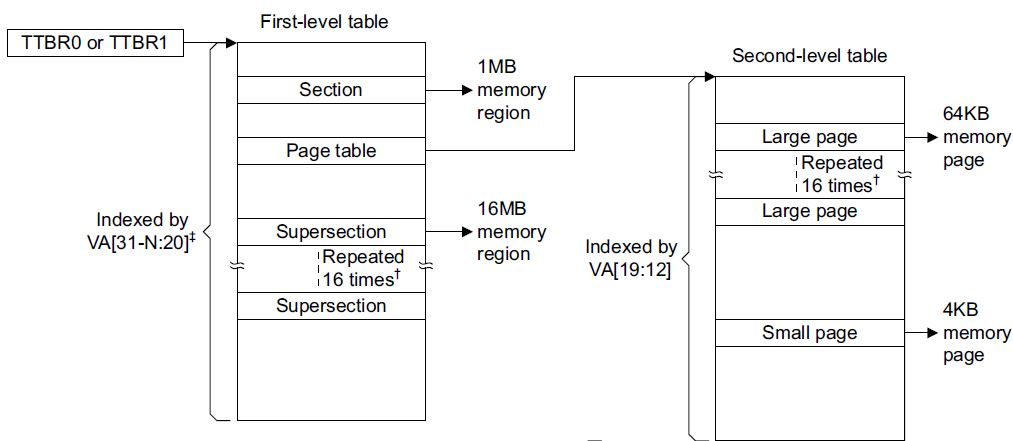
\includegraphics[scale=0.7]{chapters/mmu/figures/addressTranslation}
	\caption{Zweistufiges Seitentabellensystem \cite[S. B3-1325]{ARM:ARM}}
	\label{fig:2levelTableSystem}
\end{figure}


\subsection{Umwandlung virtueller Adressen zu physikalische Adressen}

Der genaue Vorgang der Umwandlung einer vom \textit{ARM}-Prozessor erzeugten virtuellen Adresse in eine physikalische Speicheradresse zeigen die nachfolgenden beiden Abbildungen. Abbildung  \ref{fig:sectionTranslation} zeigt die Umwandlung einer virtuellen Adresse in die physikalische Adresse einer $1MB$ Section ohne Verwendung einer Level-2-Seitentabelle, Abbildung \ref{fig:smallPageTranslation} diejenige einer virtuellen Adresse in ein $4kB$ \textit{Page Frame} unter Verwendung einer Level-2-Seitentabelle. Die Umwandlung wird vollständig durch die Prozessor-Hardware durchgeführt.\\


\begin{figure}[H]
	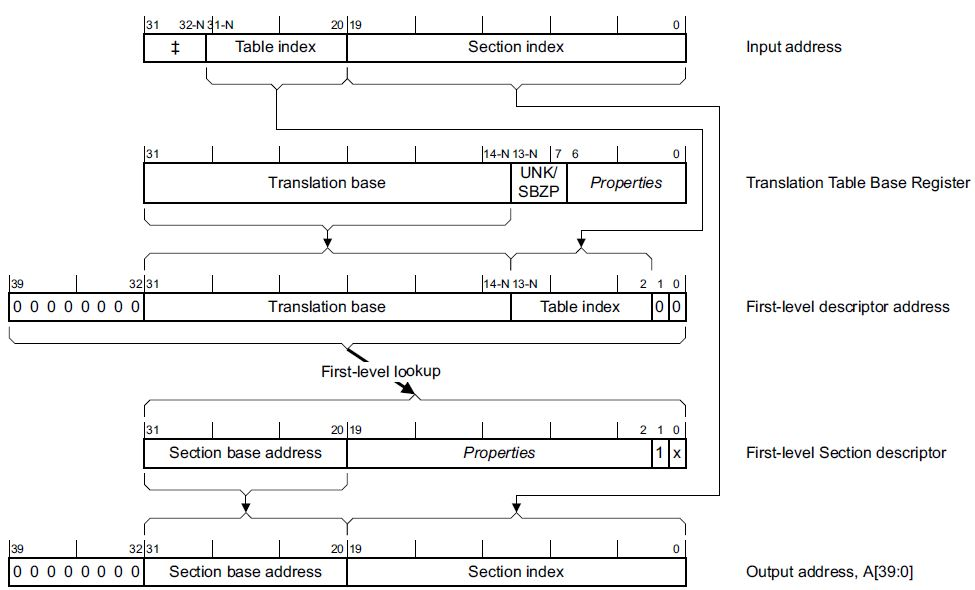
\includegraphics[scale=0.8]{chapters/mmu/figures/sectionTranslation}
	\caption{1 MB Section Translation durch die ARM CPU \cite[S. B3-1335]{ARM:ARM}}
	\label{fig:sectionTranslation}
\end{figure}

\begin{figure}[H]
	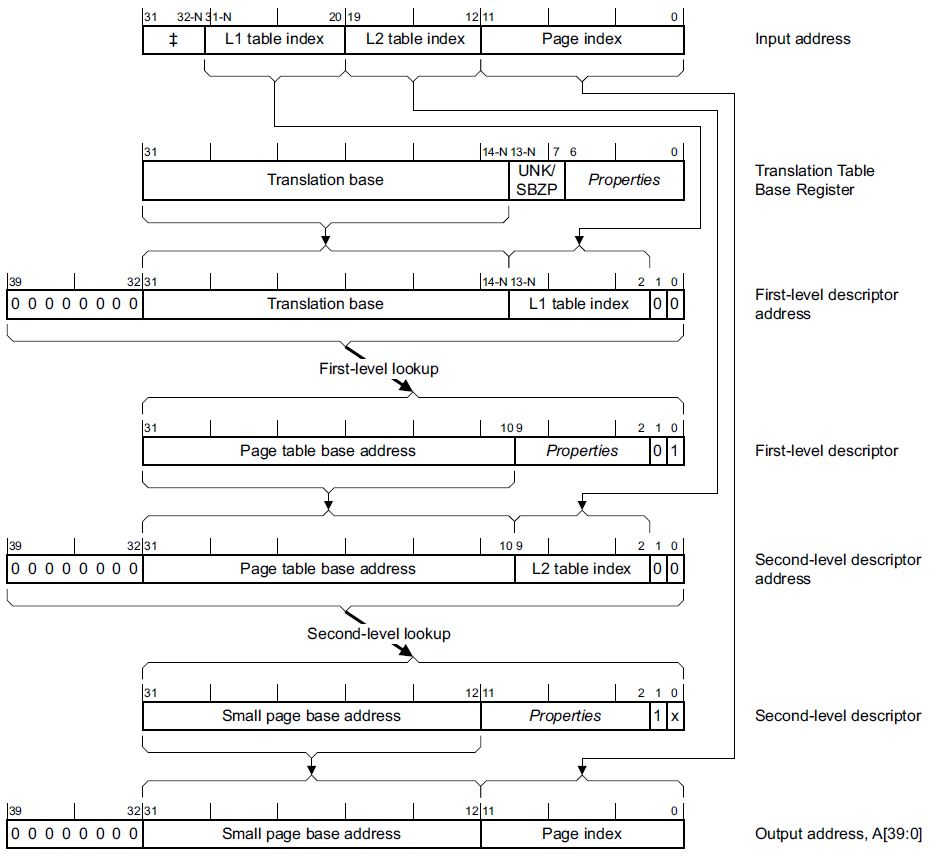
\includegraphics[scale=0.8]{chapters/mmu/figures/smallPageTranslation}
	\caption{Small Page Translation durch die ARM CPU \cite[S. B3-1337]{ARM:ARM}}
	\label{fig:smallPageTranslation}
\end{figure}

\subsection{Seitentabellen und Seitentabelleneinträge}
\label{subsect:pageTables}

Der verwendete \textit{ARM}-Prozessor verfügt über zwei Register (\acf{TTBR}, \textit{TTBR0} und \textit{TTBR1}), welche Startadressen von Seitentabellen enthalten  \cite[S. B3-1320]{ARM:ARM}. Ihre Formate sind nahezu identisch und in den Abbildungen \ref{fig:TTBR0Format} und \ref{fig:TTBR1Format} zu sehen. Diese Register übernehmen im Betriebssystem die folgende Funktion:

\begin{itemize}
	\item TTBR0: Wird für prozessspezifische Adressen verwendet. Jeder Prozess enthält bei seiner Initialisierung eine eigene Level-1-Seitentabelle. Bei einem Kontextwechsel erhält das \textit{TTBR0} eine Referenz auf Level-1-Seitentabelle des neuen Kontexts/Prozesses.
	\item \textit{TTBR1}: Wird für das Betriebssystem selbst und für \textit{Memory-Mapped I/O} verwendet. Diese ändern sich bei einem Kontextwechsel nicht.
\end{itemize}


\begin{figure}[H]
	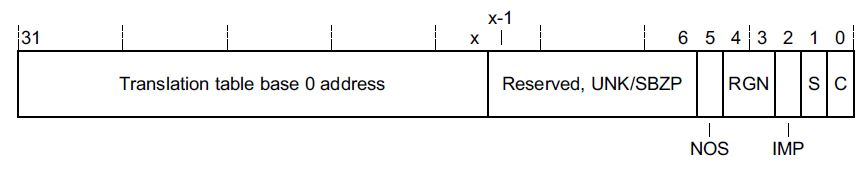
\includegraphics[scale=0.8]{chapters/mmu/figures/ttbr0format}
	\caption{TTBR0 Format \cite[S. B4-1726]{ARM:ARM}}
	\label{fig:TTBR0Format}
\end{figure}


\begin{figure}[H]
	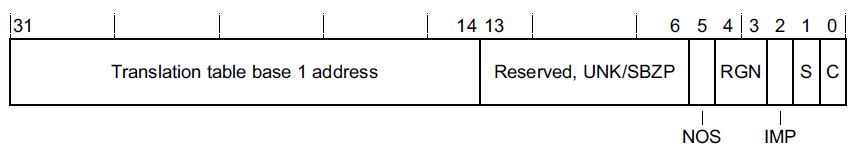
\includegraphics[scale=0.8]{chapters/mmu/figures/ttbr1format}
	\caption{TTBR1 Format \cite[S. B4-1730]{ARM:ARM}}
	\label{fig:TTBR1Format}
\end{figure}

Das Beschreiben der Seitentabellenregister erfolgt, wie bei nahezu jeder \ac{MMU}-Funktionalität, mittels Assemblerbefehlen, die auf die CP15-Coprozessor-Register zugreifen.\\

Beim Füllen der Seitentabellen sind vorgegebene Formate für die beiden Typen von Deskriptoren unbedingt zu beachten. Die Abbildungen \ref{fig:firstLevelDescriptor} und \ref{fig:secondLevelDescriptor} fassen die Formate für \textit{First-Level}- und \textit{Second-Level}-Deskriptoren zusammen. Beiden Deskriptortypen gleich ist die vorgeschriebene Länge von $32$ Bit.\\

\subsubsection*{First-Level-Deskriptoren}

Die \textit{First-Level}-Deskriptortypen werden auf folgende Weise verwendet:

\begin{itemize}
	\item \textit{Sections} für die \ac{MPT} (siehe Abschnitt \ref{subsect:memoryMapping}) 
	\item \textit{Page Table} für Level-1-Seitentabellen von Prozessen (siehe Abschnitt \ref{subsect:memoryMapping})
\end{itemize}

Für die Erstellung von \textit{First-Level}-Deskriptoren wurde eine Struktur erstellt, welche in Listing \ref{codeFirstLevelDescriptor} aufgeführt ist. Diese Struktur und jene des \textit{Second-Level}-Deskriptors wird bei den nachfolgenden Erläuterungen zur \ac{MMU} benötigt.\\

\begin{figure}[H]
	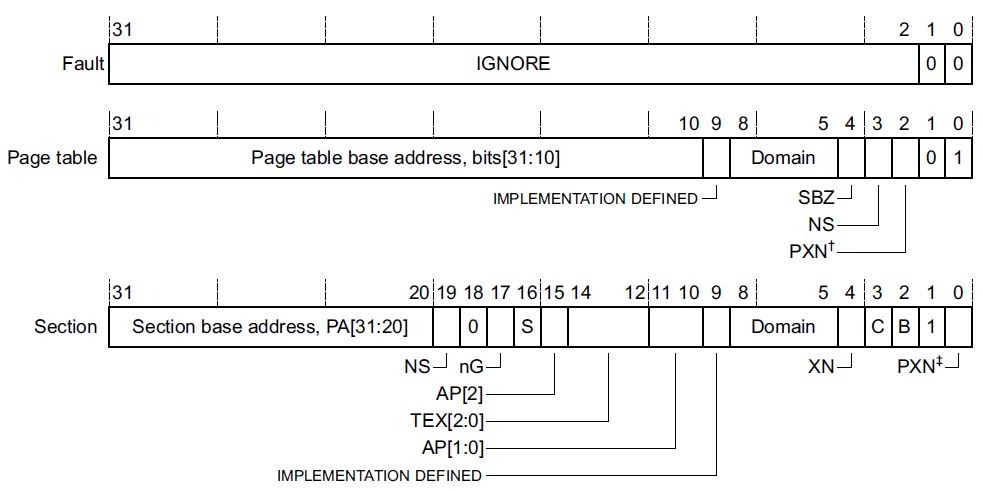
\includegraphics[scale=0.7]{chapters/mmu/figures/firstLevelDescriptor}
	\caption{First-Level Deskriptorformate \cite[S. B3-1326]{ARM:ARM}}
	\label{fig:firstLevelDescriptor}
\end{figure}


\lstinputlisting[language=C, caption=Struktur für first-level Deskriptoren, captionpos=b, label=codeFirstLevelDescriptor]{chapters/mmu/codefiles/firstLevelDescriptor.c}

\subsubsection*{Second-Level-Deskriptoren}

In der Speicherverwaltung des Betriebssystems werden ausschließlich \textit{Small Pages} verwendet. Ausschlaggebende Gründe, warum \textit{Small Pages} den Vorzug gegenüber \textit{Large Pages} erhielten, sind die folgenden:

\begin{itemize}
	\item \textit{Small Pages} müssen nur einmal in die Level-2-Seitentabelle eingetragen werden, \textit{Large Pages} hingegen 16 mal
	\item Level-1- und Level-2-Seitentabellen, die $16kB$ bzw. $1kB$ Speicher benötigen, belegen bei ihrer Erzeugung nur vier volle \textit{Page Frames} bzw. ein \textit{Page Frame} physikalischen Speichers zu einem Viertel. Dadurch wird die Speicherfragmentierung verglichen mit \textit{Large Pages} stark verringert
\end{itemize}

Die Zusammensetzung der Struktur für \textit{Second-Level}-Deskriptoren ist in Listing \ref{codeSecondLevelDescriptor} dargestellt.\\

\begin{figure}[H]
	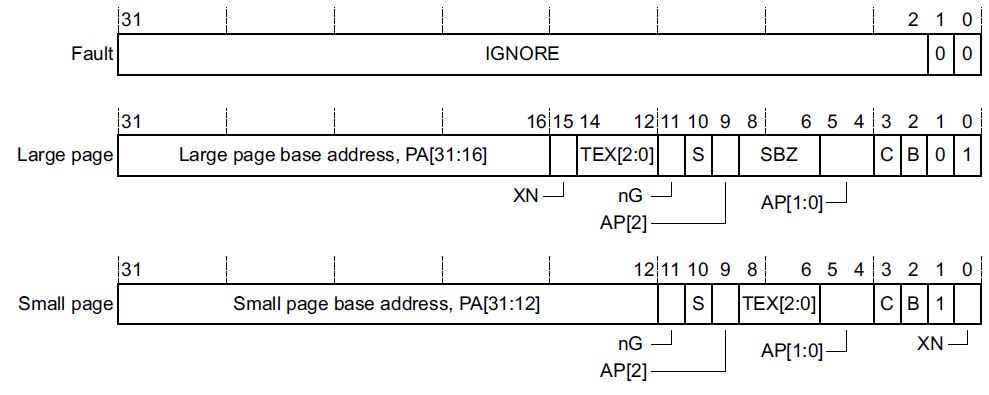
\includegraphics[scale=0.7]{chapters/mmu/figures/secondLevelDescriptor}
	\caption{Second-Level Deskriptorformate \cite[S. B3-1327]{ARM:ARM}}
	\label{fig:secondLevelDescriptor}
\end{figure}


\lstinputlisting[language=C, caption=Struktur für second-level Deskriptoren, captionpos=b, label=codeSecondLevelDescriptor]{chapters/mmu/codefiles/secondLevelDescriptor.c}


\subsection{Aufteilung des virtuellen Speichers und Mapping}
\label{subsect:memoryMapping}

Die Speicherverwaltung des Betriebssystems kann Abbildung \ref{fig:MemoryMap} entnommen werden. Die rechte Seite stellt dabei das physikalische Speichermapping dar und wurde dem Datenblatt des \textit{ARM} \cite[S. 155]{ARM:TRM} entnommen. Die linke Seite zeigt die Aufteilung des virtuellen Speichers.\\

Organisiert ist der virtuelle Speicher in Speicherregionen. Eine zusätzliche Aufteilung betrifft die Zuständigkeitsbereiche für die Seitentabellenregister \textit{TTBR0} und \textit{TTBR1}. Der \textit{ARM Cortex-A8} bietet die Möglichkeit, den virtuellen Speicher in einen Prozess- und einen Kernelbereich aufzuteilen. Der Prozessbereich enthält dabei alle virtuellen Adressen, die für Prozesse zugänglich sind. Der Kernelbereich enthält Komponenten, die sich bei Prozesswechseln nicht ändern. Dazu zählen das Betriebssystem selbst sowie die \textit{Memory-Mapped I/O}. \\ 

Die Einstellungen zur Aufteilung des virtuellen Speichers werden im \ac{TTBCR} vorgenommen. Die möglichen Aufteilungsbereiche finden sich in Tabelle B3-1, \cite[S. B3-1330]{ARM:ARM}.\\

Physikalisch steht $1GB$ Speicher für die \textit{Page Frames} zur Verfügung. Dieser wird im virtuellen Speicher an die Adressen \texttt{0x00000000} bis \texttt{0x3FFFFFFF} gemapped. Die Komponenten der Kernelregion, die sich bei Prozesswechseln nicht ändern, beginnen bei Adressen ab \texttt{0x40000000}. Damit ergibt sich eine Aufteilung des virtuellen Speichers, wie sie in Abbildung \ref{fig:MemoryMap} dargestellt ist, mit der Bereichsgrenze \texttt{0x40000000}.\\

Die Adressen ab der Bereichsgrenze bis zu den vollen $4GB$ virtuellem Speicher bei der Adresse \texttt{0xFFFFFFFF} werden in eine so genannte \textit{L1} \ac{MPT} gemapped. Bei der Aktivierung der \ac{MMU} wird die Adresse dieser \textit{Master Page Table} in das Register \textit{TTBR1} geschrieben. Danach wird \textit{TTBR1} während der Laufzeit des Betriebssystems nicht mehr verändert.\\

Bei der Initialisierung eines Prozesses wird für den Prozess eine \textit{L1 Page}, die den Prozessbereich abdeckt, angelegt. Soll ein Prozess zur Ausführung gebracht werden, muss seine \textit{L1 Page Table} in das \textit{TTBR0} geschrieben werden. Das \textit{TTBR0} muss zur Laufzeit des Betriebssystems bei Kontextwechseln von Prozessen aktualisiert werden.\\


\begin{figure}[H]
	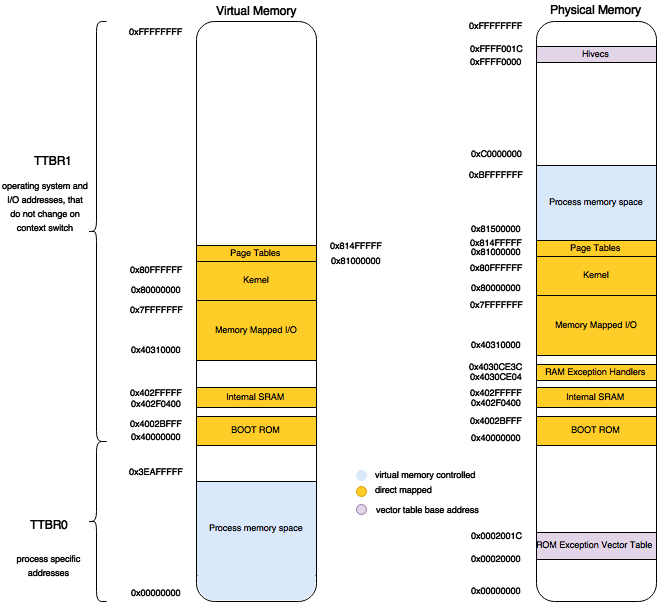
\includegraphics[scale=0.60]{chapters/mmu/figures/MemoryMap}
	\caption{Memory Map des Betriebssystems}
	\label{fig:MemoryMap}
\end{figure}

\begin{table}[H]
\begin{tabular}{p{7cm} | p{7cm}}
  \textbf{Eigenschaft} & \textbf{Beschreibung} \\ \hline
  Größe der Pages & $4kB$\\
  Virtueller Speicher für Prozesse & $1003MB$\\
  Max. Anzahl von \textit{L1} und \textit{L2 Page Tables} & $320$ \textit{L1 Page Tables} oder $1$ \textit{L1 Page Table} + $1276$ \textit{L2 Page Tables}\\
  Theoretisch Max. Anzahl von Prozessen & $320$\\
 \end{tabular}
 \caption{Eigenschaften der virtuellen Speicherverwaltung des OS}
 \label{table:SpecifiedVirtualMemory}
\end{table}

\subsubsection{Speicherregionen}

Das nachfolgende Listing \ref{codeMemoryRegion} zeigt die Struktur, mit welcher Regionen im virtuellen Speicher erstellt und verwaltet werden. Sie bieten die Möglichkeit, unterschiedlich große Bereiche des virtuellen Speichers mit denselben Eigenschaften und Zugriffsrechten zu versehen.\\

Erstellt werden solche Speicherregionen sämtliche in Abbildung \ref{fig:MemoryMap} gezeigten Bereiche. Sie enthalten die virtuelle Anfangs- und Endadresse der Region sowie Pagegröße und Zugriffsrechte auf die Region. Weiters enthalten sie eine verkettete Liste von Strukturen, die den Status(reserviert oder nicht reserviert) der einzelnen Pages verwaltet.\\

\lstinputlisting[language=C, caption=Struktur für die Verwaltung von Speicherregionen, captionpos=b, label=codeMemoryRegion]{chapters/mmu/codefiles/region.c}
\vspace{0.5cm}

Zusammengefasst dargestellt sind in Tabelle \ref{table:MemoryRegions} alle Speicherregionen des Betriebssystems. Ein direktes Mapping bedeutet dabei, dass die virtuelle Adresse der physikalischen entspricht.\\

\begin{table}[H]
\begin{tabular}{p{4cm} | p{1.5cm} | p{1.5cm} | p{6cm}}
  \textbf{Region} & \textbf{Mapping} & \textbf{Größe} & \textbf{Beschreibung} \\ \hline
  Page Tables & direkt & $5MB$ & Speicherort für L1 und L2 Page Tables\\
  Kernel & direkt & $16MB$ & Speicherort für das Betriebssystem\\
  Memory-Mapped I/O & direkt &  $1GB$ & Peripheriemodule\\
  Exception Handlers & direkt &  $4kB$ & Enthält die Exception vector table\\
  Internal SRAM & direkt & $64kB$ & Enthält die Exception handler\\
  BOOT ROM & direkt & $192kB$ & für zukünftige Erweiterungen \\ 
  Process memory space & virtuell & $1GB$ & Speicherbereich für Prozesse
 \end{tabular}
 \caption{Angelegte Speicherregionen}
 \label{table:MemoryRegions}
\end{table}


\subsubsection{Master Page Table}

Um das Mapping der \ac{MPT} verstehen zu können, wird nochmals auf den Adresstranslationsablauf in Abbildung \ref{fig:sectionTranslation} verwiesen. Alle direkt gemappten \textit{Regions} aus Tabelle \ref{table:MemoryRegions} werden in die L1 \ac{MPT} als $1MB$ \textit{Sections} gemapped.\\

Die Adresse eines Eintrags in der \textit{Page Table} setzt sich zusammen aus der Basisadresse der entsprechenden \textit{Page Table} und einem Index. Nach dem setzen der Attribute des \textit{Page-Table}-Eintrags wird durch die Funktion \texttt{MMUGetTableIndex} aus den obersten Bits der physikalischen Adresse der Index in der \textit{Page Table} berechnet. Der Index muss um $2$ Bit nach links geshiftet werden, um das \textit{Alignment} von $4$ Byte einzuhalten. Schließlich wird der geshiftete Index noch durch die Datentypgröße von $4$ Byte geteilt. Damit wird die korrekte Adresse des zu schreibenden Tabelleneintrags durch Pointerarithmetik ermittelt. An diese Adresse wird nun der Eintrag geschrieben, der zuvor durch die Funktion \emph{MMUCreateL1PageTableEntry} aus der übergebenen \textit{First-Level}-Deskriptorstruktur erstellt wurde. Listing \ref{codeMasterPageTableMapping} zeigt die praktische Ausführung des direkten Mappings in die \ac{MPT}.\\ 


\lstinputlisting[language=C, caption=Funktion für direktes Mapping in die master page table, captionpos=b, label=codeMasterPageTableMapping]{chapters/mmu/codefiles/directMapIntoMasterPageTable.c}

\subsection{Allokierung der Page Frames}

Für die Verwaltung der \textit{Page Frames} wurde eine Bitsmap verwendet. Abbildung \ref{fig:BitsMap} zeigt das Prinzip.
Die Bitsmap wird durch ein Array der Länge $N/8$ Bytes realisiert. $N$ steht hier für die Anzahl der page frames. Das $i$-te Bit im $n$-ten Byte der Bitsmap definiert den Verwendungsstatus des $(n*8 + i)$–ten \textit{Page Frame}.

\begin{figure}[H]
	\centering
	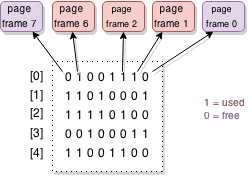
\includegraphics[scale=1]{chapters/mmu/figures/BitsMap}
	\caption{Beispiel einer Bitsmap zur Verwaltung der Page Frames}
	\label{fig:BitsMap}
\end{figure}

\subsubsection{Allokation von Page Frames bei Data Abort Exception}

Der Vorgang der Einlagerung von \textit{Page Frames} durch den \textit{Data Abort Handler} ist in Abbildung \ref{fig:dabthandler} dargestellt. Zuerst werden aus dem \ac{DFSR} der Fehlerzustand und aus dem \ac{DFAR} die zugegriffene virtuelle Adresse geladen. Eine Liste aller möglichen Fehlerzustände kann unter \cite[B3-1415]{ARM:ARM} eingesehen werden.

Ohne Ausnahme wird bei allen Zustände außer den Zuständen 5 und 7 der jeweilige Prozess beendet. Zustand betrifft die Erstellung einer \textit{L2 Page Table} und die Einlagerung eines \textit{Page Frame}. Zustand 7 betrifft die bloße Einlagerung eines \textit{Page Frame}. Die Einlagerung der \textit{Page Frames} erfolgt dabei auf sehr ähnliche Weise wie in Listing \ref{codeMasterPageTableMapping} vorgenommen.

\begin{figure}[H]
	\centering
	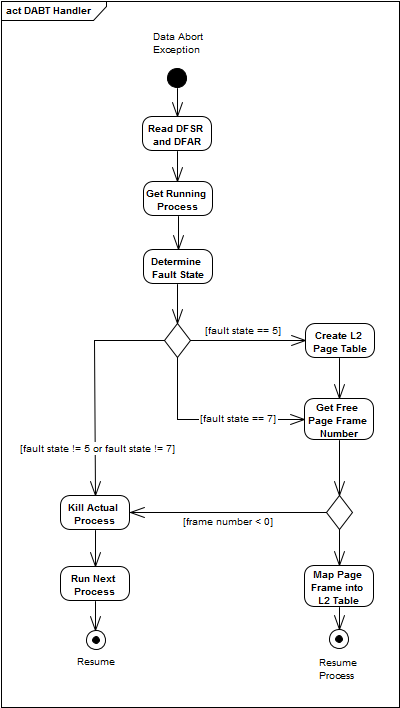
\includegraphics[scale=0.75]{chapters/mmu/figures/DABTHandler}
	\caption{Einlagerung von page frames duch den DABT-Handler}
	\label{fig:dabthandler}
\end{figure}


\subsection{Aktivieren der MMU}
\label{subsect:activateMMU}

Bevor die \ac{MMU} erfolgreich aktiviert werden kann, muss vorher eine Reihe von Einstellungen gesetzt werden.\\


Listing \ref{codeMMUInit} zeigt den kompletten Ablauf zur Aktivierung der \ac{MMU}.

\lstinputlisting[language=C, caption=Aktivierung der MMU, captionpos=b, label=codeMMUInit]{chapters/mmu/codefiles/MMUInit.c}


\subsection{Interaktion der MMU mit Prozessen}

Die Schnittstelle des \textit{MemoryManagers}, welche die \ac{MMU}-Funktionalitäten implementiert, zeigt Listing \ref{codeMMUFunctions}.\\

\lstinputlisting[language=C, caption=Softwareschnittstelle der MMU und des MemoryManagers, captionpos=b,  label=codeMMUFunctions]{chapters/mmu/codefiles/MMUFunctions.c}
\vspace{0.5cm}

Die Schnittstellenfunktionen werden auf die folgende Weise verwendet: 

\begin{description}
	\item[\texttt{MMUInit}] \hfill \\ Initialisiert die Regionen des virtuellen Speichers und die MMU für die Verwendung. Nach dem Ausführen dieser Funktion ist die MMU eingeschaltet. Bei nach erfolgreichem Ausführen wird als Rückgabewert 1 zurückgeliefert. Diese Funktion wird bei der Initialisierung des Prozess Managers aufgerufen.
	\item[\texttt{MMUSwitchToProcess}] \hfill \\ Bringt den als Parameter übergebenen Prozess zur Ausführung. Dabei wird der TLB geflusht und die Adresse der L1 page table des Prozesses in das TTBR0 geschrieben. 
	\item[\texttt{MMUInitProcess}] \hfill \\ Erstellt beim Erzeugen eines neuen Prozesses eine L1 page table für diesen Prozess. Die page table wird mit fault entries initialisiert.
	\item[\texttt{MMUHandleDataAbortException}] \hfill \\ Diese Funktion wird bei jeder Data Abort Exception ausgeführt. Sie wird durch einen in Assembler implementierten Dabt Handler aufgerufen. Die Funktion lädt die virtuelle Adresse, bei deren Zugriff die Data Abort Exception ausgelöst wurde aus dem \acf{DFAR} sowie den Fehlerstatus aus dem \acf{DFSR}. Die weitere Vorgehensweise wird in Abhängigkeit vom Fehlerstatus durchgeführt.
	\item[\texttt{MMUFreeAllPageFramesOfProcess}] \hfill \\ Beim Killen eines Prozesses gibt diese Funktion sämtliche von diesem Prozess belegten page frames in der zur Verwaltung der page frames eingesetzten Bitsmap wieder frei.
\end{description}

Die Funktionen des \textit{MemoryManagers} selbst werden ausschließlich von oben angeführten Funktionen verwendet.

\pagebreak 